%%%%%%%%%%%%%%%%%%%%%%%%%%%%%%%%%%%%%%%%%%%%%%%%%%%%%%%%%% 
\section{はじめに}
%%%%%%%%%%%%%%%%%%%%%%%%%%%%%%%%%%%%%%%%%%%%%%%%%%%%%%%%%% 

%%%%%%%%%%%%%%%%%%%%%%%%%%%%%%%%%
\begin{figure*}[t]
  \centering
  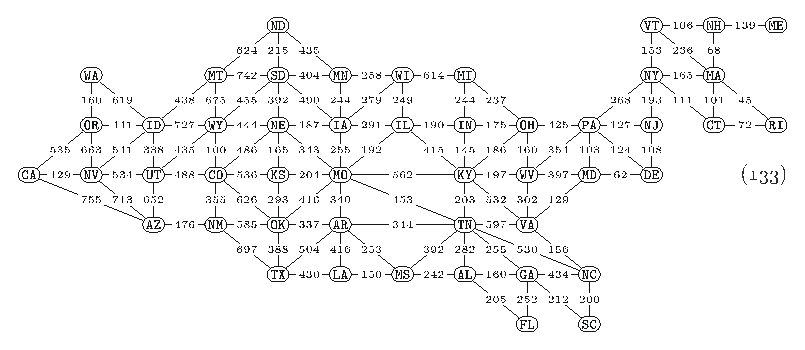
\includegraphics[width=0.7\linewidth]{fig/taocp_vol4fasc1b_p52_eq133.pdf}
  \caption{D.~E.~Knuth の教科書にある米国本土48州の隣接関係を表すグラフ}
  \label{fig:USmap}
\end{figure*}
%%%%%%%%%%%%%%%%%%%%%%%%%%%%%%%%%


\textbf{ハミルトン閉路問題} (Hamiltonian Cycle Problem; HCP) は,
与えられたグラフの全頂点をちょうど一度ずつ通る閉路が存在するかどうかを
判定する問題である\cite{hirata15:book}.
ハミルトン閉路問題は代表的な NP 完全問題である.
\textbf{ハミルトン路問題} (Hamiltonian Path Problem; HPP) は,
ハミルトン閉路問題から始点と終点が一致するという閉路の条件を取り除いた
ものである.
これらの問題は,重要な工学的応用が数多く存在するため,古くから盛んに研
究されている.
例えば,数理最適化の分野で有名な巡回セールスマン問題は,グラフの辺に距
離が付随しているとき,最短距離のハミルトン閉路を求める
\textbf{最短ハミルトン閉路問題}と考えることができる.
また,ごく最近では,距離の総和が所与の閾値以下(または以上)であることを
制約条件として付加した
\textbf{コスト制約付きハミルトン閉路問題}
の解を高速に全列挙するアルゴリズムも提案されている\cite{comp20:Minato}.
本研究では,これらの(無向グラフ上の)ハミルトン閉路問題およびその関連問
題を対象とする.

解集合プログラミング(Answer Set Programming; ASP\cite{%
  Baral03:cambridge,%
  Gelfond88:iclp,%
  Inoue08:jssst,%
  Niemela99:amai})
は,論理プログラミングから派生した宣言的問題解法のための
プログラミングパラダイムである.
ASP言語は,一階論理に基づく知識表現言語の一種である.
論理プログラムは ASP のルールの有限集合である.
ASP システムは論理プログラムから安定モデル意味論に基づく解集合を計算す
るシステムである.
近年,SAT技術を応用した高速 ASP システムが開発され,
スケジューリング,
プランニング,
システム生物学,
システム検証
%制約充足問題,
%制約最適化問題
など様々な分野への実用的応用が急速に拡大している.
%
ハミルトン閉路問題およびその関連問題に対して ASP を用いる利点としては,
ASP 言語の高い表現力,
高速な解列挙,
組込み非閉路制約,
充足不能コアに基づく最適化,
インクリメンタルASP解法
などが挙げられる.

本論文では,解集合プログラミング(ASP)を用いた
ハミルトン閉路問題,
最短ハミルトン閉路問題,
コスト制約付きハミルトン閉路問題
の解法について述べる.
%
ハミルトン閉路問題を解くASP符号化として,
\textsf{undirected},
\textsf{directed},
\textsf{acyclicity}
の3つを考案した.
\textsf{undirected}は,
ハミルトン閉路問題を次数制約と連結制約で簡潔に表現した符号化である.
\textsf{directed}は,
与えられた無向グラフの各辺$u-v$に対して,
2つの弧$u\rightarrow v$と$v\rightarrow u$を対応させることで有向グラフ
化して解く符号化である.
% 変換した有向グラフ上のハミルトン閉路は元の無向グラフ上のハミルトン閉路
% となり,また逆も成り立つ.
\textsf{acyclicity}は,\textsf{directed}符号化をベースに,
連結制約に代わる部分閉路禁止制約を,
ASP の組込み非閉路制約~\cite{bomanson16:acyclicity}で表現した符号化である.
最短ハミルトン閉路問題とコスト制約付きハミルトン閉路問題については,
考案した3つの符号化に目的関数とコスト制約をそれぞれ追加することで自然
に拡張できる.

考案した符号化の有効性を評価するために,
Flinders Hamiltonian Cycle Project (FHCP) で公開されている
HCPインスタンス(全1001問)~\cite{haythorpe19:fhcp}を用いて実験を行った.
この問題集は FHCP Challenge と呼ばれる国際競技会で使用された
頂点数が 66個から9,528個の HCP インスタンスから構成されている.
実験の結果,
\textsf{directed}符号化が 875 問と最も多くの問題を解き,
他の符号化と比較してその優位性が確認できた.


%%% Local Variables:
%%% mode: latex
%%% TeX-master: "paper"
%%% End:
